% Multiple Choice Question 3
\begin{center}
    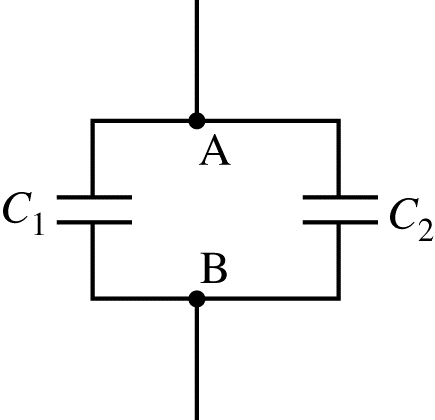
\includegraphics[scale=0.3]{images/img-003-001.png}
\end{center}

\begin{questions}
\setcounter{question}{2}

\question
Capacitors $C_{1}$ and $C_{2}$ are connected as shown in the circuit above. The capacitance of $C_{1}$ is $C$, and the capacitance of $C_{2}$ is $C / 3$. The equivalent capacitance between points $\mathrm{A}$ and $\mathrm{B}$ is $C_{\mathrm{EQ}}$. A dielectric is inserted into capacitor $C_{2}$, and the equivalent capacitance between points $A$ and $B$ is now $2 C_{\mathrm{EQ}}$. What is the value of the dielectric constant for this dielectric?

\begin{choices}
    \choice $2$
    \choice $3$
    \choice $4$
    \choice $5$
    \choice The value cannot be determined without knowing the value of $C$.
\end{choices}

\end{questions}
